\documentclass[border = 120pt]{standalone}

\usepackage[landscape]{geometry}
\usepackage{tikz}
\usetikzlibrary{mindmap}
\usepackage{metalogo}
\usepackage{dtklogos}
\begin{document}
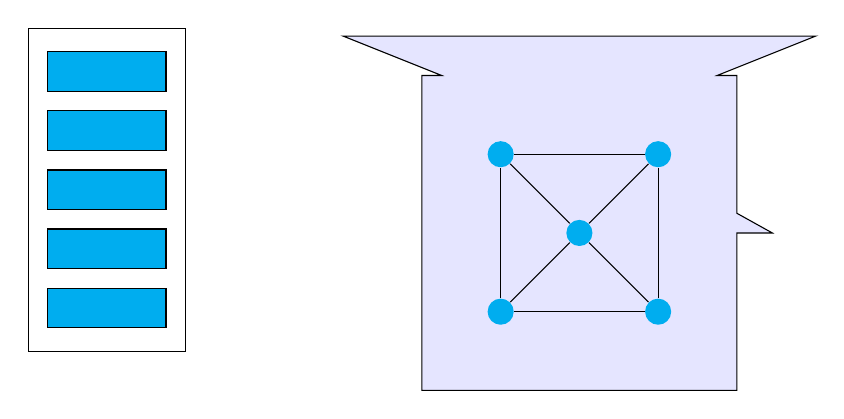
\begin{tikzpicture}

%Mother Ship
%\draw[fill=blue!10] (-8,0) rectangle (-10, 3);
%\draw[style=thick, fill=cyan] (-9.75, 2) rectangle (-8.25, 2.5);

%Jupyter Box
\draw[fill=white] (-10, 4.1) rectangle (-8, 0);
\draw[fill=cyan] (-9.75, 3.8) rectangle (-8.25, 3.3);
\draw[fill=cyan] (-9.75, 3.05) rectangle (-8.25, 2.55);
\draw[fill=cyan] (-9.75, 2.3) rectangle (-8.25, 1.8);
\draw[fill=cyan] (-9.75, 1.55) rectangle (-8.25, 1.05);
\draw[fill=cyan] (-9.75, 0.8) rectangle (-8.25, 0.3);

% Second machine
\path[draw, fill=blue!10] (-5, -0.5) -- (-5, 1.5) -- (-5, 3.5) -- (-4.75, 3.5) -- (-6, 4) -- (0, 4) --(-1.25, 3.5) -- (-1, 3.5) -- (-1, 1.75) -- (-0.55, 1.5) -- (-1, 1.5) -- (-1, -0.5) -- cycle;

// Nodes
\tikzstyle{every node} = [circle]
\node[fill=cyan] (a) at (-4, 0.5) { };
\node[fill=cyan] (b) at (-2, 0.5) { };
\node[fill=cyan] (c) at (-2, 2.5) { };
\node[fill=cyan] (d) at (-4, 2.5) { };
\node[fill=cyan] (e) at (-3, 1.5) { };
\foreach \from/\to in {a/b, b/c, c/d, a/d, a/e, e/b, c/e, d/e}
\draw [-] (\from) -- (\to);

\end{tikzpicture}
\end{document}















